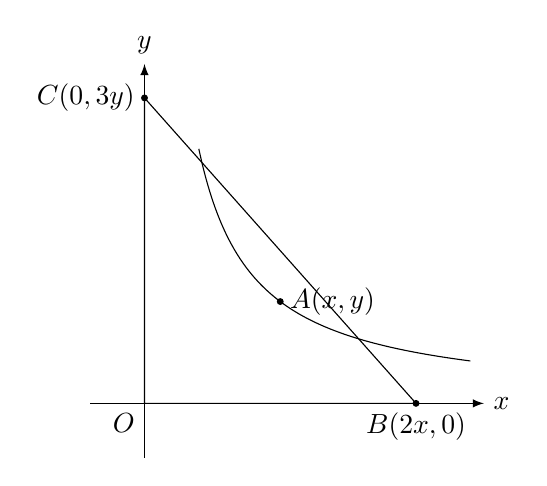
\begin{tikzpicture}[scale=0.8621,>=latex]
  \draw[->] (-0.8,0)--(5,0) node[right]{$x$};
  \draw[->] (0,-0.8)--(0,5) node[above]{$y$};
  \node[below left] at (0,0){$O$};
  \draw[smooth,domain=0.8:4.8,samples=80] plot(\x,{3/\x});
  \coordinate (A) at (2,1.5);
  \coordinate (B) at (4,0);
  \coordinate (C) at (0,4.5);
  \draw (0,0)--(B)--(C)--cycle;
  \fill (A) circle(1.45pt) node[right]{$A(x,y)$};
  \fill (B) circle(1.45pt) node[below]{$B(2x,0)$};
  \fill (C) circle(1.45pt) node[left]{$C(0,3y)$};
\end{tikzpicture}
